\documentclass{article}
\usepackage{arxiv}
\usepackage[utf8x]{inputenc}
\usepackage[english]{babel}
% \usepackage[T2A, T1]{fontenc}
\usepackage{url}
\usepackage{booktabs}
\usepackage{amsfonts}
\usepackage{nicefrac}
\usepackage{microtype}
\usepackage{lipsum}
\usepackage{graphicx}
\usepackage{natbib}
\usepackage{doi}
\usepackage{amsmath,amsfonts,amssymb,amsthm,mathtools}
\usepackage{caption}
\usepackage{float}
\usepackage{subcaption}

%\usepackage{subfigure}
\DeclareMathOperator*{\argmax}{\arg\!\max}
\DeclareMathOperator*{\argmin}{\arg\!\min}



\title{Improving algorithmic alignment with autoregressive memory}

\author{Nikita Okhotnikov\\
	\texttt{okhotnikov.nv@phystech.edu} \\
}
\date{}

\renewcommand{\shorttitle}{\textit{arXiv} Template}

\hypersetup{
pdftitle={A template for the arxiv style},
pdfsubject={q-bio.NC, q-bio.QM},
pdfauthor={Nikita Okhotnikov},
}


\begin{document}
\maketitle
\begin{abstract}
    ...
\end{abstract}

\section{Introduction}
    ....

     Consider a $\mathcal{G}(f, X)$ -- symmetry group generated
    by an algorithm $f:~ X\to Y$, a group of all transformations of elements of $X$ under which $f$ is equivariant. With such a definition, network being trained to 
    mimic an algorithm $f$ for input set $X$ can be seen as implicitly learning a set of symmetries from $\mathcal{G}(f, X)$. NAR \cite{velivckovic2021neural} 
    pipeline heavily relies on learning classical algorithms and most of them have quite a lot of symmetries. Thus, to expect reasonable performance we must embody 
    some of the known symmetries directly into the architecture as a natural constraint to narrow the optimization set. This is the main reasong why 
    permutation equivariant networks with some structural alignment with the data are used for NAR processors. 
    Similarly, that is why hint prediction approach is a typical baseline for that task. However, those predefined algorithm steps represent not the symmetry
    of the data itself, but just one possible way to apply $f$ to the input in a sequential human-readable manner. Therefore, this direct step-following 
    training manner might not be optimal. 

    The most common choices for the processor network architecture for NAR are message-passing GNNs. As GNN is applied to all the vertices simultaneously 
    it's more likely to be better at learning vertex-parallelizable steps rather than mimicking the path-following-like classical graph algorithms' steps. 
    This is another reason why a more general and less constrained approach might exist. 

\section{Related Work}
    ...
\subsection{Algorithmic alignment}
    Previously known approaches follows the mathematical idea presented in \cite{xu2019can}.
    It relies on the definition of algorithmic alignment. Consider the following notaion: \\
    $\mathcal{D}$ -- data distribution, $\{x_i, y_i\}_{i=1}^M$ -- i.i.d samples from $\mathcal{D}$, $\exists g: g(x_i) = y_i$\\ 
	$\varepsilon > 0$ -- error parameter, $\delta \in (0,1)$ -- error probability\\
	$\mathcal{A}: 2^\mathcal{D} \to \{f| f: \mathcal{X}\to \mathcal{Y}\}$ -- learning algorithm, that generates mapping function by given samples\\

	Definition 1 (Function learnability):\\
		Assume $\varepsilon >0 $, $\delta\in (0,1)$, $\{x_i, y_i\}_{i=1}^M$ are chosen and $y_i = g(x_i)$ for some $g$. \\
		Let $f = \mathcal{A}(\{x_i, y_i\}_{i=1}^M)$ be the function generated by a learning algorithm $\mathcal{A}$.
		Then $g$ is $(M, \varepsilon, \delta)$-learnable with $\mathcal{A}$ if 
		$$\mathbb{P}_{x\sim \mathcal{D}}\left[\|f(x)-g(x)\|\leq \varepsilon\right] \geq 1-\delta$$ \\

	Definition 2 (Sample complexity):\\
		Sample complexity $\mathcal{C}_\mathcal{A}(g, \varepsilon, \delta)$ is the minimum $M$ so that $g$
		is $(M, \varepsilon, \delta)$-learnable with $\mathcal{A}$.\\

    Definition 3 (Algorithmic alignment):\\
        Assume $\mathcal{N}$ is neural network with $n$ modules $\mathcal{N}_i$. \\
        Let $g: \mathcal{X} \to \mathcal{Y}$ be a reasoning function. \\
        Module functions $f_1, \dots, f_n$ generate $g$ for $\mathcal{N}$ if, by replacing $\mathcal{N}_i$ with $f_i$, the network $\mathcal{N}$ simulates $g$.\\ 
        Then $\mathcal{N}$ $(M, \varepsilon, \delta)$-algorithmically aligns with $g$ if $f_1, \dots, f_n$ generate $g$ and 
        there are learning algorithms $\mathcal{A}_i$ for the $\mathcal{N}_i$ such that $n\cdot\max_i C_{\mathcal{A}_i}(f_i, \varepsilon, \delta)\leq M$.\\	

    
    Theorem 1:\\ 
        $\mathcal{A}$ -- an overparameterized and randomly initialized 2-layer MLP trained with GD for a sufficient number of iterations.
        Suppose $g:~\mathbb{R}^d\to \mathbb{R}^m$ with components $g(x)^{(i)} = \sum_j \alpha_j^{(i)} \left(\beta_j^{(i)\top}x\right)^{p_j^{(i)}}$, where
        $\beta_j^{(i)}\in \mathbb{R}^d,~\alpha\in\mathbb{R}$ and $p_j^{(i)} = 1$ or $p_j^{(i)} = 2l,~(l\in \mathbb{N})$. 
        Then the sample complexity $\mathcal{C}(g, \varepsilon, \delta)$ is 
        \[\mathcal{C}_\mathcal{A}(g, \varepsilon, \delta) = O\left( \frac{\max_i\sum_{j=1}^{K} p_j^{(i)}|\alpha_j^{(i)}|\cdot\|\beta_j^{(i)}\|_2^{p_j^{(i)}} + \log (m / \delta)}{(\varepsilon / m)^2} \right)\]

    Theorem 2:\\
        For some $\varepsilon, \delta$ suppose $\{S_i, y_i\}_{i=1}^M\sim \mathcal{D}, ~|S_i|< N,~ y_i = g(S_i)$ for some $g$. 
        Suppose $\mathcal{N}_1\dots \mathcal{N}_n$ are sequential MLP modules of $\mathcal{N}$. Suppose $\mathcal{N}$ and $g$ $(M, \varepsilon, \delta)$-algorithmically align via $f_1\dots f_n$.	
        Then $g$ is $(M, O(\varepsilon), O(\delta))$-learnable by $\mathcal{N}$.\\
    
    Corollary 1:\\
        Suppose universe $S$ has $n$ objects $x_1\dots x_n$ and $g(S) = \sum_{i,j} (x_i - x_j)^2$. Then the sample complexity 
        of MLP is $O(n^2)$ times larger than that of GNN.
    

\section{ExtraARM-GNN}
We suggest an extra \textit{Auto-Regressive Memory} (ARM) to be added to the model instead of <<hints>>, that stores an \textit{<<idea>>} representation on each 
individual step for later use (after being generated, <<idea>> remains unchanged to the very end). To enforce step-by-step <<thinking>> and ideas captioning, we 
use the same idea of contrastive self-supervised constraint as in \cite{rodionov2024neural} and \cite{bevilacqua2023neural}, but instead of matching the 
intermediate representation of the nodes, we match the ARM and take a not different steps, but different inputs as hard-negatives. That allows model 
to discover different ways of approximating the algorithm not forcing it to follow the same steps, but forcing to grasp and store the same sequence 
of graph features for similar inputs. To implement ARM in auto-regressive manner we can utilize self-attention mechanism along with binary 
attention mask in a way similar to transformer language models decoders \cite{vaswani2023attentionneed}, unmasking new idea-token on each step.

Let us denote by $M_t(X) \in \mathbb{R}^k$ the idea generated on step $t$ for input $X$, then $M(X)\in \mathbb{R}^{k\times T}$ --- is a concatenation
 of all the ideas and the state of the ARM after the last processor step. Sticking to the notation used in \cite{rodionov2024neural}, 
 $\mathcal{X}$ is the set of possible inputs, $\mathcal{X}_X\subset \mathcal{X}$ --- the set of inputs considered similar to $X$,
 $\overline{\mathcal{X}_X}\subset \mathcal{X}$ --- the set of inputs considered non-similar to $X$ 
 (negatives, on practice can be sampled randomly as from $\mathcal{X}$ for each batch)

\textbf{Note:} as the architecture has become less constraint, we can consider wider classes of inputs <<similar>>
 than ones of an identical trajectory. Moreover, we can train the same architecture simultaneously for different algorithms 
 sharing similar steps as in \cite{ibarz2022generalist} or for primal-dual algorithm pairs as in \cite{numeroso2023dual} as 
 we are not anymore bound with the necessity to predict the actual steps of a classical algorithm on each step.

With notation from the above, the resulting contrastive constraint is as follows:

$$L = - \sum_{X\in \mathcal{X}}\sum_{X_a \in \mathcal{X}_X}\log\frac{  \exp{\left(  \sum_{t=1}^{T} \phi\left(M_t(X), M_t(X_a)\right)  \right)}  }{  \exp{\left(  \sum_{t=1}^{T} \phi\left(M_t(X), M_t(X_a)\right)  \right)} + \sum\limits_{\overline{X_a}\in \overline{\mathcal{X}_X}}\exp{\left(\sum_{t=1}^{T}\phi\left(M_t(X), M_t(\overline{X_a})\right)\right)}  }$$

where $\phi$ is a proximity function.

Suggested processor network architecture sketch is shown on \ref{fig1}.

\begin{figure}[h!]
    \centering
        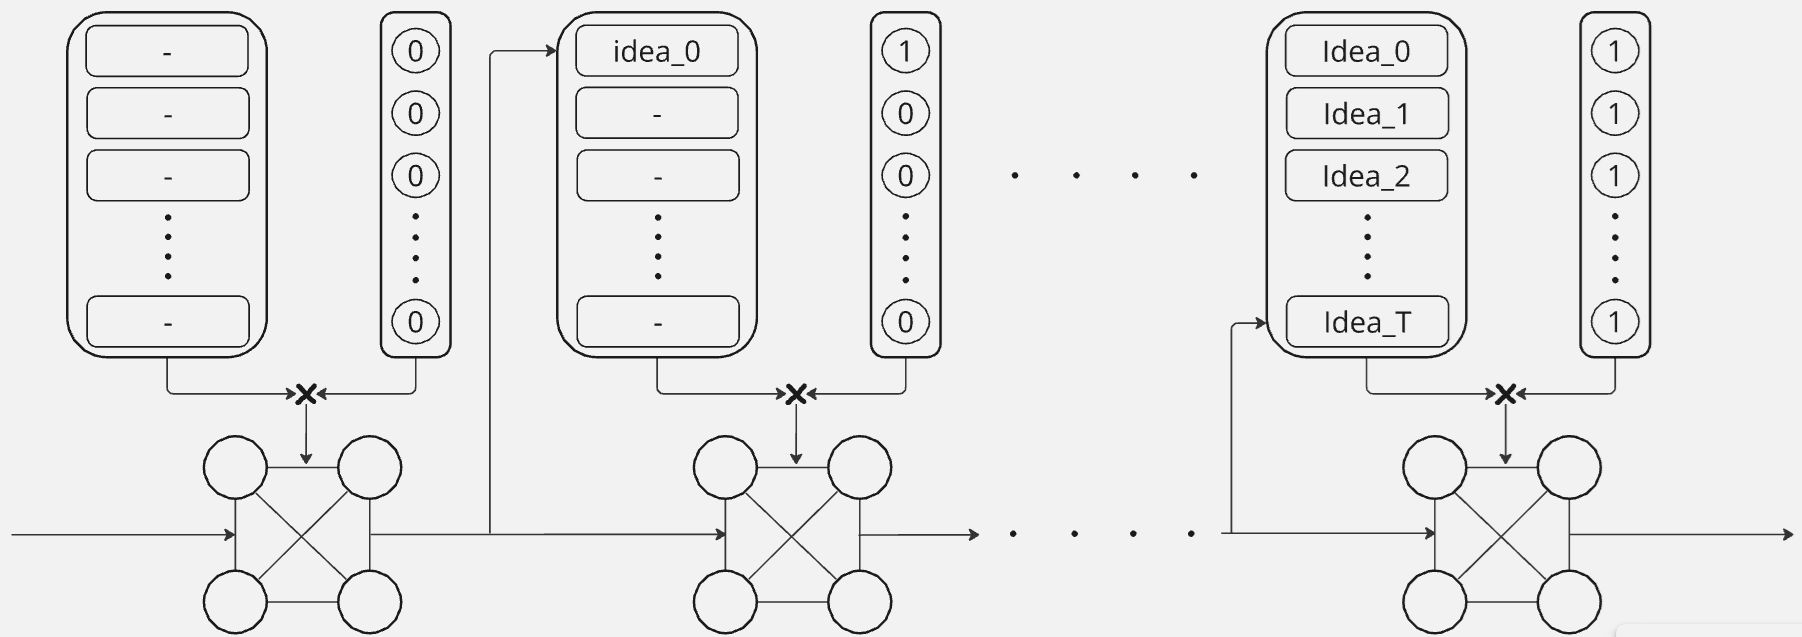
\includegraphics[scale=0.35]{../pictures/extra-ARM-GNN.png}
    \caption{Architecture}
    \label{fig1}
\end{figure}

\section{Experiments}
    ... 
\section{Conclusion}
    ...




\bibliographystyle{plain}
\bibliography{references.bib}

\end{document}